\documentclass[final,11pt]{article}
\usepackage{times}
\usepackage{epsfig}
\usepackage{multirow} 
\usepackage[left=.80in,top=.85in,right=.80in,bottom=.85in]{geometry}
% 14.5 pages:
% \usepackage[left=.78in,top=.74in,right=.78in,bottom=.75in]{geometry}
% lots of margin:
% \usepackage[left=1.00in,top=1.00in,right=1.00in,bottom=1.00in]{geometry}
\usepackage{subfig}
\usepackage{wrapfig}
\usepackage{enumerate}
\usepackage{afterpage}
\usepackage{sectsty}
\usepackage{enumitem}
\usepackage{colortbl} 
\usepackage{comment}
\usepackage{graphicx}
\usepackage{setspace}
%\usepackage{bibspacing}
\usepackage{url}
%\usepackage{gensymb}
%\usepackage{pgfgantt}
\usepackage{amssymb}
\usepackage{nicefrac}

\newif\ifcmm
\cmmfalse
\long\def\CMM#1{
\ifcmm #1\else\relax\fi}
\def\thechapter{./}
\usepackage{moreepsf}
\long\def\AuthorNote#1{%
{\Large\bf #1}}
\def\Action#1{\texttt{#1}}
\def\TiC{{\sc corc}}

\definecolor{purple}{rgb}{.6,.2,.4} 
\definecolor{ltblue}{rgb}{.6,.6,1}

\newcommand{\ignore}[1]{ }
\graphicspath{{./}{figures/}} 

\newcommand{\defn}[1]{\textbf{\textit{#1}}}
\renewcommand{\emph}[1]{\textbf{\textit{#1}}}

% Shrink space in enums and lists
\setlist{topsep=3pt,itemsep=3pt,parsep=3pt}
\setlist[1]{labelindent=\parindent}

% Bolded figure captions in the ACM style
\makeatletter
\long\def\@makecaption#1#2{%
   \vskip 10\p@
   \setbox\@tempboxa\hbox{{\bf#1: #2}}%
   \ifdim \wd\@tempboxa >\hsize
    {\bf #1: #2}\par
     \else
       \hbox to\hsize{\hfil\box\@tempboxa\hfil}%
   \fi}
\makeatother


% Make bullet list singled spaced
\newenvironment{packed_item}{
\begin{list}{\labelitemi}{%
  \leftmargin=1.0em
  \setlength{\itemsep}{3pt}
  \setlength{\parskip}{0pt}
  \setlength{\parsep}{3pt}
}
}{\end{list}}

\def\paragraph#1{%

\smallskip

\noindent{\bf #1}\hbox to 1em{\hss}%
}

\newenvironment{rquote}{\setlength{\leftmargini}{1em}\setlength{\leftmarginii}{1em}\quotation\noindent}{\endquotation}

% Make enumberated list singled spaced
\newenvironment{packed_enum}{
\begin{enumerate}
  \setlength{\itemsep}{1pt}
  \setlength{\parskip}{0pt}
  \setlength{\parsep}{0pt}
}{\end{enumerate}}



% Modify the default section and subsection headers
\makeatletter
\def\@seccntformat#1{\@ifundefined{#1@cntformat}
{\csname the#1\endcsname\,}
{\csname #1@cntformat\endcsname}
}
\def\section@cntformat{\thesection.\,}
\def\subsection@cntformat{\thesubsection.\,}
\def\subsubsection@cntformat{\thesubsubsection.\,}

%phjones changed to 1, 2, 2.1 ...
%\def\thesection{\Roman{section}}
%\def\thesubsection{\thesection.\Alph{subsection}}
%\def\thesubsubsection{\thesubsection.\arabic{subsubsection}}
%\makeatother

%phjones changed to 1, 2, 2.1 ...
\def\thesection{\arabic{section}}
\def\thesubsection{\thesection.\arabic{subsection}}
\def\thesubsubsection{\thesubsection.\arabic{subsubsection}}
\makeatother

\sectionfont{\normalsize\MakeUppercase}
\subsectionfont{\normalsize}


% Create a non-indented bolded start to a paragraph.
\newcommand{\npara}[1]{\noindent{\bf #1}}


% Increase the space between paragraphs.
\setlength{\parskip}{.8ex plus 0.5ex minus 0.2ex} 


%for comments
\newcommand{\FIXME}[1]{\textcolor{red}{FIXME: #1}}

\pagestyle{empty}
\begin{document}
\thispagestyle{empty}
\setcounter{page}{0}

\begin{center}
{\Large Catoptric Systems for Managing Light}

\vskip 0.2in
{\sc Roger Chamberlain, Chandler Ahrens, Chris Gill}
\\Dept. of Computer Science and Engineering, McKelvey School of Engineering\\
College of Architecture, Sam Fox School of Design \& Visual Arts
\\Washington University in St.~Louis
\vskip 0.05in
{\sc Abby Stylianou}
\\Dept. of Computer Science, College of Arts and Sciences
\\Saint Louis University
\vskip 0.05in
{\sc Malia Gehan}
\\Donald Danforth Plant Science Center
\vskip 0.05in
Email: roger@wustl.edu


\end{center}

\clearpage
\pagestyle{plain}
\setcounter{page}{1}
\pagenumbering{arabic}

\section{Introduction}
\label{sec:intro}

%\FIXME{Here is a reference to make sure that citations are working~\cite{Bugbee16,bblmw19}.}

Energy consumption due to buildings (both residential and commercial)
is estimated to be 20\% to 40\% of the total energy usage in
developed countries~\cite{pop08}, and
lighting and heating are two significant components of this demand~\cite{keh05}.
Natural light (i.e., sunlight) is a readily available resource that
can contribute both to the illumination~\cite{Leslie03}
and to the heating~\cite{Lunde80} of structures.
Further, the use of natural light for plant growth is dramatically more
energy efficient than artificial lighting~\cite{Bugbee16}.
For example, supplemental lighting at the Donald Danforth Plant Science Center
greenhouses consumes over 4~million~kWh per year at a cost upwards of
\$350,000 annually.

We propose to investigate how to utilize actively
controlled catoptric (mirror) surfaces effectively for improved
plant growth, illumination, and heating of buildings.  Through computer-based control of
the dynamic positioning of
individual mirrors, and cyber-physical integration of the mirrors,
the devices
that orient them, and customized objectives and
constraints,
we propose to enable fine-grained management of sunlight as a resource.

Figure~\ref{fig:amp} shows a prototype catoptric surface (called AMP) that was 
designed, fabricated, and installed during an undergraduate architecture studio 
taught by Co-PI C.~Ahrens. The installation redirects light from gable ends of an 
existing building into the darker recesses of the atrium.
We next developed a
new version in which over 600 mirrors are under 
active, 2-axis control and therefore the mirrors
can be pointed in different directions dynamically as desired over
time~\cite{acmbg19,acmb18,cagm18}. 
This next-generation installation is within 
the south wall of the Steinberg Hall atrium on the campus of 
Washington University; a subset of the mirrors in this new
installation is shown in Figure~\ref{fig:steinberg}.

\begin{figure}[ht]
\centering
\subfloat[\mbox{ }]{
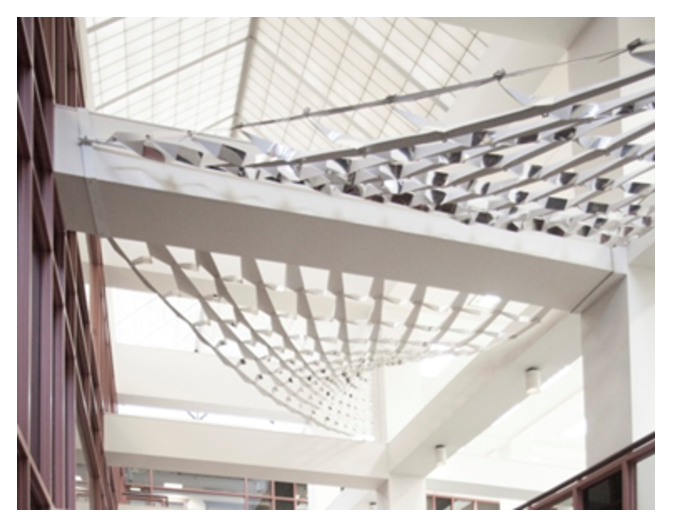
\includegraphics[width=0.45\linewidth]{figures/amp}
\label{fig:amp}}
\qquad \qquad
\subfloat[\mbox{ }]{
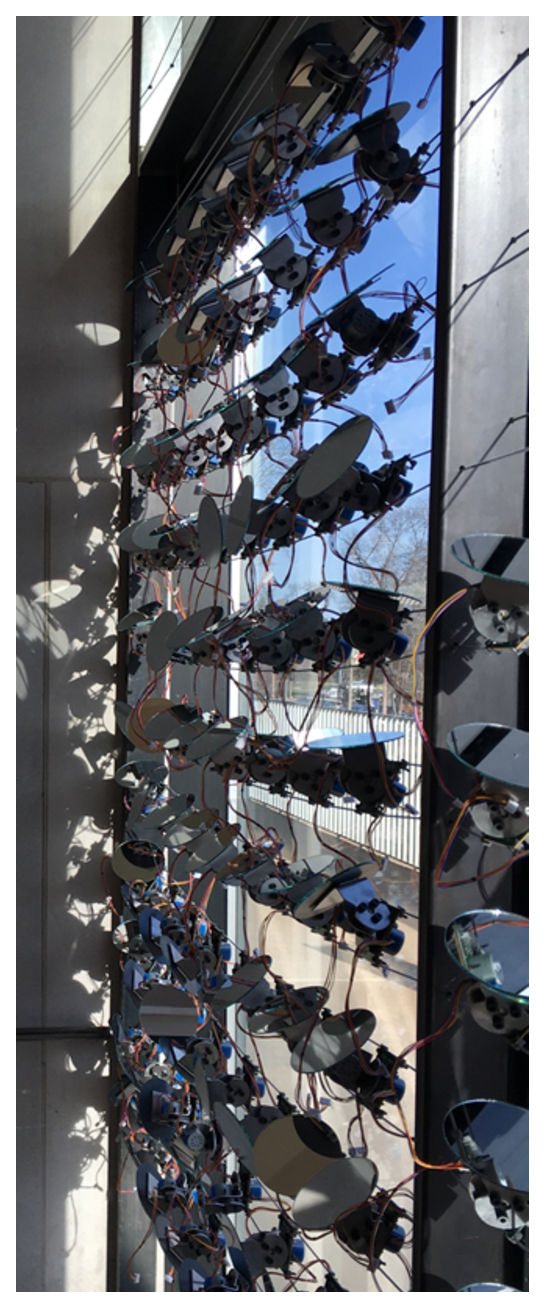
\includegraphics[width=0.14\linewidth]{figures/steinberg}
\label{fig:steinberg}}
\caption{Catoptric system prototypes.
(a)~\emph{AMP}, TRex building, St.~Louis.
(b)~Steinberg Hall, St.~Louis.
}
\label{fig:proto}
\end{figure}

The community with which we will partner on this effort is
the 39~North AgTech Innovation District in St.~Louis County. Under the
supervision of the county and the St.~Louis Economic Development Partnership, 
a master plan has been prepared to develop the area in the vicinity of  
anchor institutions Bayer AG and the Donald Danforth Plant Science Center. 
This includes greenspaces, startup incubators, redesigned roadways, etc.,
all in support of new agriculture technology businesses and plant science.

\section{Integrative Research}
\label{sec:research}

\FIXME{Outline the technical and social science concepts and planning
activities, including potential for transferability and scalability.}

Through this proposed research, we will advance the state of the art in
catoptric systems, using two important applications to guide and evaluate the
development of prototype systems: sustainable and controlled plant growth,
and lighting
and thermal management of human-occupied buildings\footnote{No human subjects
research will be conducted as part of the planning grant. Any subsequent
research
that includes human subjects will be under the supervision of the IRB at
Washington University.}.
Our proposed investigations
will target three primary objectives: (1) identifying and quantifying benefits
that can be achieved by redirecting light (including daylight, incandescent
light, light from LEDs, and combinations thereof) for 
plant growth (i.e., food production),
building lighting, and thermal management, through the use of
catoptric systems; (2) establishing and evaluating models and methods to ensure
the safety, reliability, maintainability, and continued efficacy of these
systems, using rigorous methods based in Markov Decision Processes for modeling
and policy generation; and (3) extracting common abstractions from the
instantiation and evaluation of the approach in three distinct application
domains (food production, building lighting, and building HVAC), as a starting
point for further application of the approach in other smart and connected
communities applications.

\subsection{Intellectual Merit}
\label{sec:im}

In addition to projected broader impacts on community nutrition, illumination
of occupied spaces, and sustainable energy use, this proposed research is of
significant intellectual merit in expanding and deepening the kinds of
cyber-physical systems capabilities that are pertinent to smart and connected
communities. Specifically, by introducing active modalities (sensing, control,
coordination, and actuation) into historically passive (daylight) or largely
static (artificial lighting) modalities, and controlling and coordinating them
with respect to well-defined objective functions in each of several distinct
applications, we seek to transform how light is used indoors.  

For example, plants growing in greenhouses often use supplemental artificial
light. Artificial lighting is energetically expensive and examining the
effectiveness of redirecting natural light in comparison to
(and possibly in combination with)
artificial lighting is both largely unexamined and well aligned with the
expertise and interests of the research team.
Similarly, daylighting (the use of natural light for illumination) design is
dominated by passive window positioning and configuration~\cite{vgf+13}
rather than
active control mechanisms, except in a few cases~\cite{kt16}.
Heating systems that
exploit sunlight frequently use actively-controlled mirrors for tracking the
relative position of the sun, but there is limited experience with using the
same sets of mirrors for both thermal and lighting control.

We propose to investigate how to utilize actively controlled catoptric (mirror)
surfaces effectively for improved food production and illumination and heating
of buildings. Through computer-based control of the dynamic positioning of
individual mirrors, and cyber-physical integration of natural and artificial
light sources, the mirrors, the devices that orient them, and customized plant
growth, building lighting and heating objectives and constraints, we propose to
enable adaptive and fine-grained management of light as a resource throughout a
building.

We propose to develop image-based maps as the primary tool for understanding
the incident light in indoor scenes. Prior to the catoptric interventions,
these maps would highlight where light is concentrated based on visual
observation and knowledge of the scene geometry and lighting (natural and
artificial). We then intend to use candidate maps that indicate where light is
desired to determine the necessary configuration of the smart mirror array. We
propose two approaches by which such candidate maps can be generated: first, we
will develop interfaces for users to create their own candidate maps indicating
where in the scene they desire additional lighting; second, we intend to
explore the use of deep learning approaches to scene and human activity
understanding~\cite{chao:wacv2018,Gkioxari_2018_CVPR,Redmon2015YouOL,Toshev_2014_CVPR}
to generate candidate maps of where light would be most
effectively redirected (e.g., using deep learning approaches to detect where a
person is in a scene, and to understand the task that they are performing, in
order to determine the most appropriate candidate lighting conditions).


Given the desire to control different combinations light (sunlight and
different sources of artificial light) via catoptric surfaces, for different
plant growth, illumination and/or thermal management objectives, a number of
crucial cyber-physical systems issues must be addressed.  For example, we will
investigate how existing techniques like multi-objective control be applied to
manage the relationships among potentially competing goals within each
application (which themselves also will be articulated and quantified as a
contribution of this proposed research). We also intend to investigate whether
Markov Decision Process (MDP) models can serve as a cohesive framework within
which each application domain's distinct multi-objective control problem can be
represented, and appropriate control policies generated automatically (e.g.,
through techniques like policy iteration), recognizing that maximization of an
objective function in expectation is a robust way to acknowledge the inherent
uncertainty of future events (whether it be sunlight availability, lighting
demand, or any other effect that is either stochastic in nature or is
sufficiently complex but stationary so that it can be modeled as such).

Constraints for safety, reliability, and maintainability, also will be modeled,
alongside the objective functions for the continued efficacy of a catoptric
system in each particular application domain.  Even with a suitable
multi-objective control approach in place, it is essential that such
requirements are all addressed together, at once, and consistently. For
example, considering safety: highly concentrated sunlight could be damaging
either to a plant or a person and so would lead to deterioration of the
expected value for the objective function in food production or illumination
applications.  However, in a HVAC application, such light aimed at a heat
collector (important when harvesting energy for thermal management purposes)
may need to be limited even if its increase would improve the application's
objective function, as it could be harmful to a person who inadvertently
contacted the beam of light.  This example in turn reveals the kinds of nuances
that may be in play for such systems, which in turn may inform other
cyber-physical applications - for example detecting the presence or absence of
a person in that scenario could inform sensing, control, and actuation
decisions.  Reliability and maintainability considerations similarly may span
both objective functions and constraints, for example in community food
production settings where failure of the system would impair vital nutritional
resources on which a community increasingly relies.

An important feedback mechanism we will investigate is the use of visual
data (imagery and video) for assessing the safety, reliability, and
efficacy of catoptric systems. This will include determination of the true
orientation of each mirror, providing information on the available
light and its current positioning, as well as providing feedback on
benefits to both plants and humans.
In particular, we will investigate different sensing modalities (e.g., RGB,
thermal) for understanding both the safety of an implemented smart mirror
configuration, as well as measuring observable benefits in the scene (e.g.,
visual metrics of plant health such as greenness or leaf temperature).

\subsection{Research Questions}
\label{sec:rq}

\FIXME{Detail technological and social science research questions, hypotheses
and research gaps that will be explored during the planning period.}

Several key considerations for this proposed research will be the effectiveness
and ease with which: (1)~abstract state representations (within the MDPs) can
adequately track and manage complex real-world applications, (2)~large numbers
of mirrors, sensors, and pan-tilt units can be managed over long periods of
time as some of them may degrade or cease functioning entirely, and
(3)~fundamental issues with observability that arise from the first two
considerations.  We propose to address the first consideration through careful
abstraction of each application domain's most salient features within our
models.  In the domain of food production, we will 
identify and/or define initially simplified
models for how different illumination patterns may optimize food growth.
For example, mirrors might be positioned to optimize light penetration
through the canopy.
We will then apply those models to control catoptric surfaces in small-scale
physical experiments, and refine the models based on the results of those
studies.

The second consideration will be addressed by tracking and reporting
the potential degradation of individual elements in the prototype test-bed we
will develop for each application domain, and examining the uncertainty in
sensing, actuation, and control that may occur because of it.  Incorporating
uncertainty into our MDP-based models, e.g., through developing POMDP models,
PAC bounds (as we have done in prior work~\cite{gtgs10}),
and other methods will be another important contribution of this
research.

The third consideration is centered around observability. 
This includes investigating how deep learning approaches to scene and
human activity recognition can be used to automatically understand where
lighting modifications are necessary in scenes, and 
assessing the safety and ``success'' of the catoptric systems
(emotion or behavior recognition plus human-in-the-loop feedback
in office environments, thermal measurements in HVAC systems,
visual measurements of plant health and productivity).


\section{community Engagement}
\label{sec:community}

\FIXME{We have current connections with the Donald Danforth Plant Science
Center (a collaborating organization) and two commercial firms
(VelociData, Inc.\footnote{\url{http://www.velocidata.com}} and
BECS Technology, Inc.\footnote{\url{http://www.becs.com}}).}

\begin{figure}[ht]
\centering
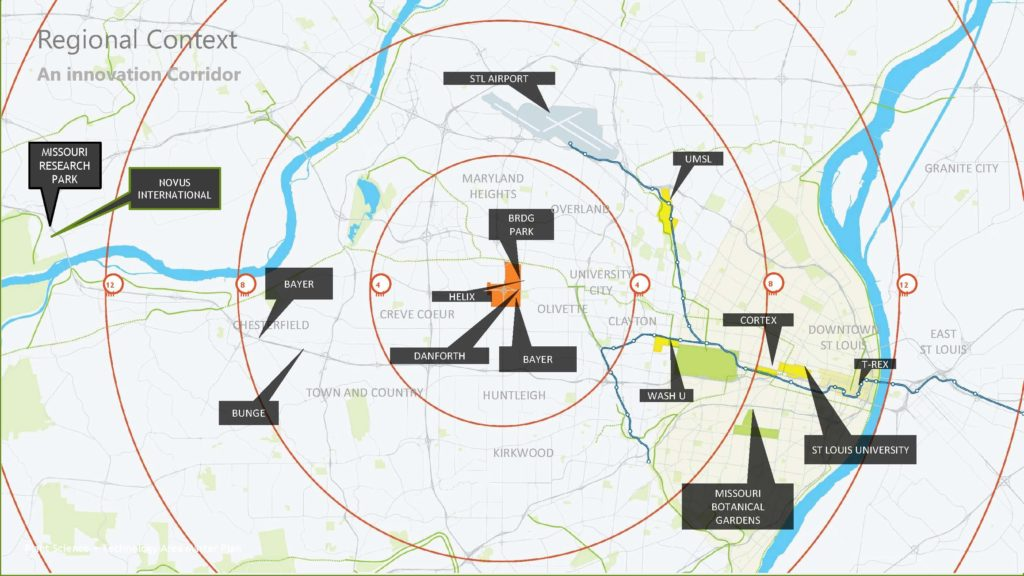
\includegraphics[width=0.75\linewidth]{figures/39N}
\caption{39 North is in the center of a regional AgTech innovation corridor.}
\label{fig:39N}
\end{figure}

\section{Broader Impacts}
\label{sec:broader}

The proposed research is expected to have important impacts on the built environment.
According to the EPA, buildings are responsible for producing 6\% of
greenhouse gasses and heat and electrical generation produces another
25\%\footnote{\url{https://www.epa.gov/ghgemissions/global-greenhouse-gas-emissions-data}}.
A large portion of the electrical consumption in buildings is used for
heating, cooling and artificial lighting. Our proposal addresses the
reduction of electricity for artificial lighting to be replaced by
reflected daylight and capturing the solar heat. During daytime hours,
daylight is a preferred source of light for many people and the proposal
directs the daylight deeper into a building. The daylight reflection system
provides a more sustainable approach by reducing the required electricity
and provides a more desirable quality of light.

\FIXME{Talk about nutrition and plants. Malia, can you provide some text that
makes sense here?}

\section{Results from Prior NSF Support}
\label{sec:prior}

Co-PI C. Ahrens has not had prior NSF funding. The projects described
below are representative examples of NSF-supported research led by PI 
R.~Chamberlain and co-PI C.~Gill.

%\noindent
{\large\bf CSR: Small: Concurrent Accelerated Data Integration}
{\bf (CNS-1527510,
PI R. Chamberlain)}, 
10/2015--9/2019, \$519,275.  
%
\textbf{Intellectual Merit} -- This project is investigating the
accelerated execution of data integration workflows, which
increasingly are bottlenecks in data science. Execution platforms
include both graphics engines and FPGAs.
%
\textbf{Broader Impacts} -- This project has supported 5
graduate and 6 REU students.  The applications investigated
come from biology, astrophysics, and the IoT,
further expanding the scope of the students'
experience.
%
\textbf{Evidence of Research Products and their Availability} --
Publications resulting from this work include~\cite{cc19,dibs,c17,fcbmc19,mgc16,js16}.
A benchmark suite of the above workflows has been released
as a community resource~\cite{dibsv1}.

%\noindent
{\large\bf CPS: Medium: Collaborative: CyberMech, a Novel Run-Time Substrate for 
Cyber-Mechanical Systems}
{\bf (CNS-1136073 and CNS-1136075,
WU PI C. Gill)}, 9/2011-8/2016, \$1,800,000 total.  
%
This research project developed novel foundations for parallel real-time computing, demonstrating the first ever real-time hybrid simulation involving a thousand-degree-of-freedom structure at millisecond time scales.
%
\textbf{Intellectual Merit}~-- Results of this research include new methods for parallel real-time execution of control and simulation computations, new parallel real-time scheduling techniques and analyses, and characterization and exploitation of trade-offs involving both high computational demand and stringent timing constraints.
%
\textbf{Broader Impacts}~-- This multi-university project involved 7 PhD, 3 masters, and 7 undergraduate students, and 2 visiting scholars in highly multi-disciplinary research collaborations.  Results of this research are spurring
further advances in parallel real-time computing and natural hazards
engineering.
%
\textbf{Evidence of Research Products and their Availability}~-- Results of
this 
collaborative research appeared in 10 publications at
top-tier conferences and journals.
Data, experiment configurations, platform software, and simulation source-code 
have been published on-line. % at Washington University and Purdue University.


%\input{conclude}

\clearpage
% \begin{scriptsize}
\bibliographystyle{abbrv}
\bibliography{prop}
% \end{scriptsize}

\end{document}
